\documentclass[Arkitektur/System_main.tex]{subfiles}
\begin{document}
\subsubsection{RPiApp} \label{sec:rpiapp_application_model}
I dette afsnit beskrives software arkitekturen for Applikationen til RPi'en. Applikationen har fire hovedfunktioner:
\begin{enumerate}
    \item I2C Kommunikation mellem delenheder (Playerside, BallDispenser)
    \item Logisk controller, som styrer spillets gang og opdaterer resten af systemet
    \item WebPage grafisk grænseflade som modtager information fra brugeren
    \item Display grafisk grænseflade som udsender/viser information til brugeren. 
\end{enumerate}
Et klassediagram er blevet lavet for hele applikationen og den kan ses i figur \ref{fig:CD_RPI}. I de næste afsnit vil de enkelte klasser blive beskrevet samt tilhørende funktioner. 
\begin{figure}[H]
    \centering
    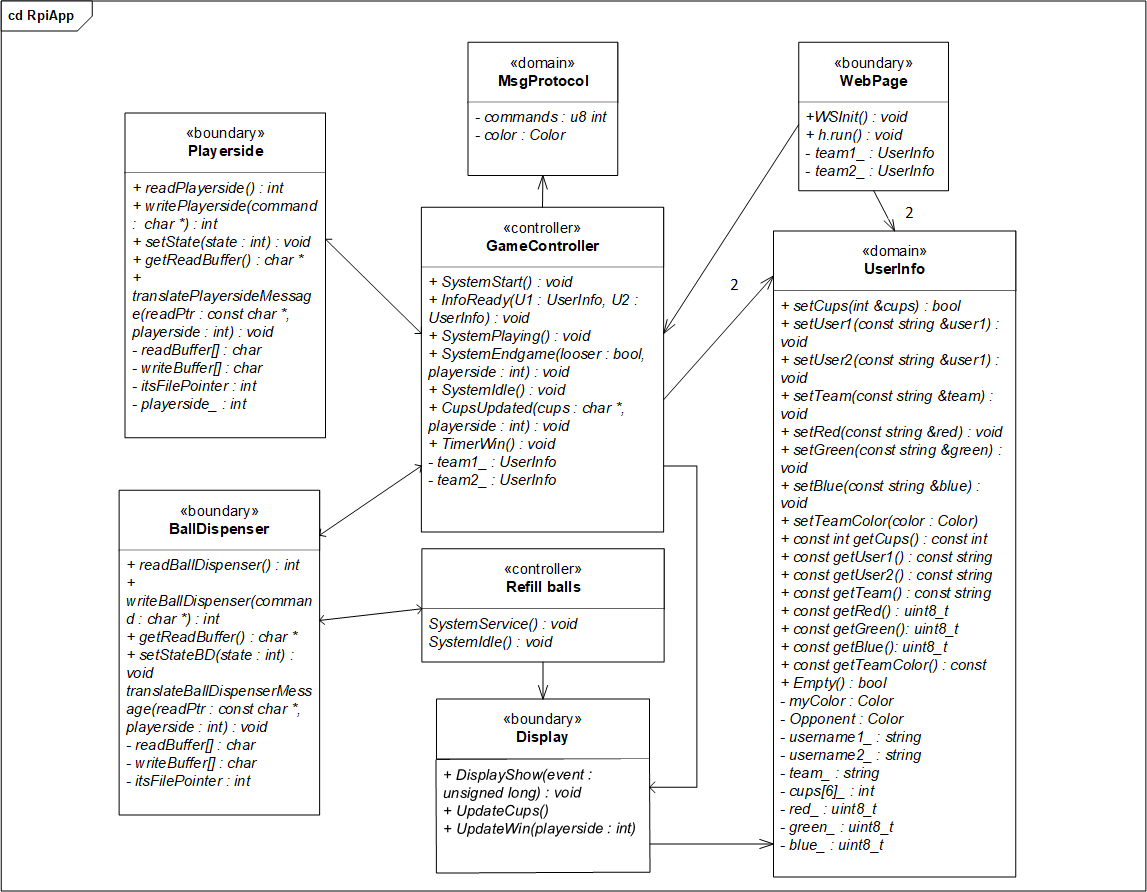
\includegraphics[width=\textwidth]{Arkitektur/Softwarearkitektur/Applikationsmodel/RPi/graphics_RPi/Class.png}
    \caption{Klassediagram for RPi}
    \label{fig:CD_RPI}
\end{figure}
\subsubsection{Funktionsbeskrivelse for RPi}
\large{\textbf{Controller:  GameController}}\\
GameController er den centrale klasse for use case 1 - 3. Den sørger for at sende og modtage data gennem klasserne BallDispenser og PlayersideRead. Alt modtaget data bliver evalueret i GameController og sendt videre i overensstemmelse med protokollen og use case flow. Klassen varetager alt logikken og de flest beslutninger i systemet.\\\\
{\large\textbf{Funktionsbeskrivelser: GameController}}\\[0.2cm]
\textbf{SystemStart() : void}
\begin{adjustwidth}{1cm}{0pt}
\textbf{Beskrivelse:} Skal sørge for at initialisere GameController klassen. Funktionen bliver kaldt når en boundary klassen 'BallDispenser' detektere en mønt. Skal derude indstille de korrekte tilstande for Playersides og BallDispenser. Alle System-operationer skal synkronisere delsystemerne.   
\textbf{Parametre:} status: ingen \\[0.2cm]
\textbf{Retur værdi:} ingen \\[0.2cm]
\textbf{Bivirkninger:} ingen \\[0.2cm]
\end{adjustwidth}
\textbf{InfoReady(U1 : UserInfo, U2 : UserInfo) : void}
\begin{adjustwidth}{1cm}{0pt}
\textbf{Beskrivelse:} Denne funktion initialisere skal initialisere team1\_ og team2\_, således de har de rigtig informationer for hvert hold. 
\textbf{Parametre:} status: U1, U2 : De to private members hos GameController som symboliserer hold.  \\[0.2cm]
\textbf{Retur værdi:} ingen \\[0.2cm]
\textbf{Bivirkninger:} ingen \\[0.2cm]
\end{adjustwidth}

\textbf{SystemPlaying() : void}
\begin{adjustwidth}{1cm}{0pt}
\textbf{Beskrivelse:} Skal indstille de korrekte tilstande for delsysterme og initiere tilstanden 'Playing' for GameController. Her skal den konstant videresende koppernes pladsering og undersøge, hvornår alle kopper er blevet fjernet. 
\textbf{Parametre:} ingen \\[0.2cm]
\textbf{Retur værdi:} ingen \\[0.2cm]
\textbf{Bivirkninger:} ingen \\[0.2cm]
\end{adjustwidth}

\textbf{SystemEndgame() : void}
\begin{adjustwidth}{1cm}{0pt}
\textbf{Beskrivelse:} Funktion som skal slutte spillet - bliver kaldt når et hold ikke har flere kopper tilbage, og det tidligere stadie har været 'Playing'.
\textbf{Parametre:} ingen \\[0.2cm]
\textbf{Retur værdi:} ingen \\[0.2cm]
\textbf{Bivirkninger:} ingen \\[0.2cm]
\end{adjustwidth}

\textbf{SystemIdle() : void}
\begin{adjustwidth}{1cm}{0pt}
\textbf{Beskrivelse:} Funktion skal sætte systemet i dvale tilstand. 
\textbf{Parametre:} ingen \\[0.2cm]
\textbf{Retur værdi:} ingen \\[0.2cm]
\textbf{Bivirkninger:} ingen \\[0.2cm]
\end{adjustwidth}

\textbf{SystemService() : void}
\begin{adjustwidth}{1cm}{0pt}
\textbf{Beskrivelse:} Skal sørge for at systemet stopper muligheden for at starte et spil indtil bolddispenseren er 'NotEmpty'. 
\textbf{Parametre:} ingen \\[0.2cm]
\textbf{Retur værdi:} ingen \\[0.2cm]
\textbf{Bivirkninger:} ingen \\[0.2cm]
\end{adjustwidth}

{\large\textbf{Attributbeskrivelser: GameController}}
\begin{adjustwidth}{1cm}{0pt}
\textbf{team1\_} Et UserInfo objekt, afspejler playerside 1 (Brugere, hold og farve) \\[0.2cm]
\textbf{team2\_} Et UserInfo objekt, afspejler playerside 2 (Brugere, hold og farve) \\[0.2cm]
\end{adjustwidth}


\large{\textbf{Boundary:  PlayerSide}}\\
Klasse til at læse/skrive til Playerside via I2C protokollen. Data/kommandoer sendes til I2CInterruptDriveren fra User Space. Klassen behandler også data modtaget fra I2CInterruptDriveren (Kernal space). 
\\\\Funktionerne "writePlayerside(..)", "readPlayerside()" og "translatePlayersideMessage(..)" kan virke lidt implicit i form er at de enten modtager en kommando gennem I2C eller videresender en prædefineret kommando. Det er altid god kodepraksis at udlicitere hvert opgave til en specifik funktion, fx "sendStateIdle()" i stedet for writePlayerside(STATE::IDLE). Den først nævnte udgave skaber højere samhørighed i det den kun har til funktion at sende stadiet "IDLE" til Playerside, hvorimod den anden funktion kan sende alt, men er afhængig af programmørens viden til protokollen. Med det sagt, så er det stadig valgt at bruge den løsning, der kræver at man kender til protokollen, da det gør klasse diagrammet mere overskueligt end 10 funktioner, som er navngivet efter hvilke information, som bliver sendt (Det samme princip gælder for BallDispenser). \\\\
\subsubsection{Funktionsbeskrivelse for RPi}
{\large\textbf{Funktionsbeskrivelser: Playerside}}\\[0.2cm]
\textbf{readPlayerside : int}
\begin{adjustwidth}{1cm}{0pt}
\textbf{Beskrivelse:} Skal læse fra Playerside enheden (Læser direkte fra en Playerside node / fil). 
Data læst skal gemmes i klassens readBuffer, samt funktionen returnere antal bytes læst. 
\textbf{Parametre:} ingen \\[0.2cm]
\textbf{Retur værdi:} Antal bytes læst  \\[0.2cm]
\textbf{Bivirkninger:} Blokerer processen og tråden indtil et interrupt modtages. \\[0.2cm]
\end{adjustwidth}

\textbf{writePlayerside(command : char *) : int}
\begin{adjustwidth}{1cm}{0pt}
\textbf{Beskrivelse:} Skal skrive til Playerside enhed (Skriver direkte til en Playerside node / fil). Returnerer 0, hvis succesful. En char sendes ad gangen til i2cInterruptDriver. 
\textbf{Parametre:} command: kommando som skal sendes (Kan fx være et stadie) \\[0.2cm]
\textbf{Retur værdi:} 0 hvis succes  \\[0.2cm]
\textbf{Bivirkninger:} ingen \\[0.2cm]
\end{adjustwidth}

\textbf{setState(state : int) : void}
\begin{adjustwidth}{1cm}{0pt}
\textbf{Beskrivelse:} Skal sætte og sende stadiet for Playerside enheden. 
\textbf{Parametre:} state: stadiet som skal indstilles for Playerside enheden \\[0.2cm]
\textbf{Retur værdi:} ingen  \\[0.2cm]
\textbf{Bivirkninger:} ingen \\[0.2cm]
\end{adjustwidth}

\textbf{getReadBuffer() : char *}
\begin{adjustwidth}{1cm}{0pt}
\textbf{Beskrivelse:} Retunere det data, som er blevet læst af readPlayerside() funktionen. 
\textbf{Parametre:} ingen \\[0.2cm]
\textbf{Retur værdi:} En char pointer til det data i readBufferen \\[0.2cm]
\textbf{Bivirkninger:} ingen \\[0.2cm]
\end{adjustwidth}

\textbf{translatePlayersideMessage(readPtr : const char *, playerside : int) : void}
\begin{adjustwidth}{1cm}{0pt}
\textbf{Beskrivelse:} Skal analysere det data som er modtaget fra Playerside enheden. Ud fra betydningen af det data, som er modtaget.
\textbf{Parametre:} readPtr: en pointer til et char array (data), playerside: hvilke Playerside/Spillerside som snakkes om; enten 1 eller 2. \\[0.2cm]
\textbf{Retur værdi:} ingen \\[0.2cm]
\textbf{Bivirkninger:} ingen \\[0.2cm]
\end{adjustwidth}

{\large\textbf{Attributbeskrivelser: Playerside}}
\begin{adjustwidth}{1cm}{0pt}
\textbf{readBuffer} Array som indeholder data læst fra Playerside enhed. \\[0.2cm]
\textbf{writeBuffer} Array med data som skal sendes til Playerside enhed \\[0.2cm]
\textbf{itsFilePointer} 'Pointer' til den specifikke fil/node associeret med Playerside enheden\\[0.2cm]
\textbf{playerside\_} indikator til hvilket Playerside enhed som klassen repræsenterer\\[0.2cm]
\end{adjustwidth}
\textbf{Boundary:  BallDispenser}\\
Klasse til at læse/skrive til BoldDispenser via I2C protokollen. Data/kommandoer sendes til I2CInterruptDriveren fra User Space. Klassen behandler også data modtaget fra I2CInterruptDriveren (Kernal space). \\\\
{\large\textbf{Funktionsbeskrivelser: BallDispenser}}\\[0.2cm]
Funktions- og attributbeskrivelse laves ikke for BallDispenser klassen beskrives ikke, da de er identiske for Playerside. Den eneste forskel er at klassen skal kommunikere med en BallDispenser enhed i stedet for en Playerside enhed. \\\\
{\large\textbf{Attributbeskrivelser: MsgProtocol}}
\begin{adjustwidth}{1cm}{0pt}
\textbf{commands} database / hukommelse om alle kommandoer og stadier, som sendes til mellem delsystemerne og hardware enhederne (fx Playerside og BallDispenser)\\[0.2cm]
\textbf{color} RGB farve type, består af 3 bytes, som definere den specifikke farve\\[0.2cm]
\end{adjustwidth}
{\large\textbf{Boundary: WebPage}}\\
Klassen udgør serversiden af hjemmesiden. Den gør brug af et WebSocket API og står for at håndtere beskeder, som modtages fra
client. Den skal initialisere to objektere af UserInfo klassen og sende dem til GameController klassen.\\
\\{\large\textbf{Attributbeskrivelser: WebPage}}
\begin{adjustwidth}{1cm}{0pt}
\textbf{team1\_} Et UserInfo objekt, afspejler playerside 1 (Brugere, hold og farve) \\[0.2cm]
\textbf{team2\_} Et UserInfo objekt, afspejler playerside 2 (Brugere, hold og farve) \\[0.2cm]
\end{adjustwidth}

{\large\textbf{Funktionsbeskrivelser: WebPage}}\\[0.2cm]
\textbf{WSInit() : void}
\begin{adjustwidth}{1cm}{0pt}
\textbf{Beskrivelse:} Skal initialisere WebSocket event handleren onMessage, som kaldes, når der modtages en besked fra client. Denne sættes til at indlæse en modtaget tekststreng i en buffer, opdele tekststrengen og gemme resultatet i en vektor. Herefter initialiseres to objekter, team1\_ og team2\_, som sendes i en besked til GameController klassens beskedkø. Endelig sendes et respons til client, for at bekræfte, at alt er forløbet korrekt.\\
\textbf{Parametre:} ingen \\[0.2cm]
\textbf{Retur værdi:} ingen \\[0.2cm]
\textbf{Bivirkninger:} ingen \\[0.2cm]
\end{adjustwidth}

{\large\textbf{Domain: UserInfo}}\\
Klassen indeholder informationer, som repræsenterer Playersides. Klassen skal således indeholde alle informationer, som er relevante for et givet hold.\\
\\{\large\textbf{Attributbeskrivelser: UserInfo}}
\begin{adjustwidth}{1cm}{0pt}
\textbf{username1\_} En tekststreng, der udgør brugernavn for spiller 1. \\[0.2cm]
\textbf{username2\_} En tekststreng, der udgør brugernavn for spillers 2. \\[0.2cm]
\textbf{team\_} En tekststreng, der udgør holdes navn. \\[0.2cm]
\textbf{cups[6]\_} Et array der angiver om kopperne er placeret eller fjernet. \\[0.2cm]
\textbf{red\_} En unsigned int, som angiver lysstyrken af det røde lys i holdet farve. Den ligger i intervallet 0-255, hvor 0 betyder slukket og 255 betyder fuld lysstyrke. \\[0.2cm]
\textbf{green\_} En unsigned int, som angiver lysstyrken af det grønne lys i holdet farve. Den ligger i intervallet 0-255, hvor 0 betyder slukket og 255 betyder fuld lysstyrke. \\[0.2cm]
\textbf{blue\_} En unsigned int, som angiver lysstyrken af det blå lys i holdet farve. Den ligger i intervallet 0-255, hvor 0 betyder slukket og 255 betyder fuld lysstyrke. \\[0.2cm]
\textbf{myColor: Color} Indeholder holdets farve.  \\[0.2cm]
\textbf{Opponent: Color} Indeholder modstanderholdets farve.  \\[0.2cm]
\end{adjustwidth}

{\large\textbf{Funktionsbeskrivelser: UserInfo}}\\[0.2cm]
\textbf{setCups(\&cups: int) : bool}
\begin{adjustwidth}{1cm}{0pt}
\textbf{Beskrivelse:} Skal sætte antallet af kopper, default er 12 kopper.\\
\textbf{Parametre:} cups: Antallet af kopper placeret i Playerside. \\[0.2cm]
\textbf{Retur værdi:} bool: True returneres, hvis der er er sat et positivt antal kopper i Playerside, ellers returneres false. \\[0.2cm]
\textbf{Bivirkninger:} ingen \\[0.2cm]
\end{adjustwidth}

\textbf{setUser1(\&user1: const string) : void}
\begin{adjustwidth}{1cm}{0pt}
\textbf{Beskrivelse:} Skal sætte brugernavnet for spiller 1.\\
\textbf{Parametre:} user1: Tekststreng som udgør brugernavnet for spiller 1. \\[0.2cm]
\textbf{Retur værdi:} ingen \\[0.2cm]
\textbf{Bivirkninger:} ingen \\[0.2cm]
\end{adjustwidth}

\textbf{setUser2(\&user2: const string) : void}
\begin{adjustwidth}{1cm}{0pt}
\textbf{Beskrivelse:} Skal sætte brugernavnet for spiller 1.\\
\textbf{Parametre:} user2: Tekststreng som udgør brugernavnet for spiller 2. \\[0.2cm]
\textbf{Retur værdi:} ingen \\[0.2cm]
\textbf{Bivirkninger:} ingen \\[0.2cm]
\end{adjustwidth}

\textbf{setTeam(\&team: const string) : void}
\begin{adjustwidth}{1cm}{0pt}
\textbf{Beskrivelse:} Skal sætte holdnavnet.\\
\textbf{Parametre:} team: Tekststreng som udgør holdnavnet. \\[0.2cm]
\textbf{Retur værdi:} ingen \\[0.2cm]
\textbf{Bivirkninger:} ingen \\[0.2cm]
\end{adjustwidth}

\textbf{setRed(\&red: const string) : void}
\begin{adjustwidth}{1cm}{0pt}
\textbf{Beskrivelse:} Skal sætte styrken af den røde farve i holdfarven.\\
\textbf{Parametre:} red: Styrken af farven rød i holdfarven. \\[0.2cm]
\textbf{Retur værdi:} ingen \\[0.2cm]
\textbf{Bivirkninger:} ingen \\[0.2cm]
\end{adjustwidth}

\textbf{setGreen(\&green: const string) : void}
\begin{adjustwidth}{1cm}{0pt}
\textbf{Beskrivelse:} Skal sætte styrken af den grønne farve i holdfarven.\\
\textbf{Parametre:} green: Styrken af farven grøn i holdfarven. \\[0.2cm]
\textbf{Retur værdi:} ingen \\[0.2cm]
\textbf{Bivirkninger:} ingen \\[0.2cm]
\end{adjustwidth}

\textbf{setBlue(\&blue: const string) : void}
\begin{adjustwidth}{1cm}{0pt}
\textbf{Beskrivelse:} Skal sætte styrken af den blå farve i holdfarven.\\
\textbf{Parametre:} blue: Styrken af farven blå i holdfarven. \\[0.2cm]
\textbf{Retur værdi:} ingen \\[0.2cm]
\textbf{Bivirkninger:} ingen \\[0.2cm]
\end{adjustwidth}

\textbf{setTeamColor(color: Color) : void}
\begin{adjustwidth}{1cm}{0pt}
\textbf{Beskrivelse:} Skal sætte holdets farve.\\
\textbf{Parametre:} color: Indeholder RGB værdier, der angiver holdets farve. \\[0.2cm]
\textbf{Retur værdi:} ingen \\[0.2cm]
\textbf{Bivirkninger:} ingen \\[0.2cm]
\end{adjustwidth}

\textbf{const getCups() : const int}
\begin{adjustwidth}{1cm}{0pt}
\textbf{Beskrivelse:} Skal returnere antallet af kopper, der er placeret i Playerside.\\
\textbf{Parametre:} ingen \\[0.2cm]
\textbf{Retur værdi:} const int: Antallet af kopper i Playerside.\\[0.2cm]
\textbf{Bivirkninger:} ingen \\[0.2cm]
\end{adjustwidth}

\textbf{const getRed() : uint8\_t}
\begin{adjustwidth}{1cm}{0pt}
\textbf{Beskrivelse:} Skal returnere en byte med styrken af farven rød i holdfarven.\\
\textbf{Parametre:} ingen \\[0.2cm]
\textbf{Retur værdi:} uint8\_t: Indholdet af farven rød i holdfarven.\\[0.2cm]
\textbf{Bivirkninger:} ingen \\[0.2cm]
\end{adjustwidth}

\textbf{const getGreen() : uint8\_t}
\begin{adjustwidth}{1cm}{0pt}
\textbf{Beskrivelse:} Skal returnere en byte med styrken af farven grøn i holdfarven.\\
\textbf{Parametre:} ingen \\[0.2cm]
\textbf{Retur værdi:} uint8\_t: Indholdet af farven grøn i holdfarven.\\[0.2cm]
\textbf{Bivirkninger:} ingen \\[0.2cm]
\end{adjustwidth}

\textbf{const getBlue() : uint8\_t}
\begin{adjustwidth}{1cm}{0pt}
\textbf{Beskrivelse:} Skal returnere en byte med styrken af farven blå i holdfarven.\\
\textbf{Parametre:} ingen \\[0.2cm]
\textbf{Retur værdi:} uint8\_t: Indholdet af farven blå i holdfarven.\\[0.2cm]
\textbf{Bivirkninger:} ingen \\[0.2cm]
\end{adjustwidth}

\textbf{const getUser1() : const string}
\begin{adjustwidth}{1cm}{0pt}
\textbf{Beskrivelse:} Skal returnere brugernavnet for spiller 1.\\
\textbf{Parametre:} ingen \\[0.2cm]
\textbf{Retur værdi:} const string: Brugernavn for spiller 1.\\[0.2cm]
\textbf{Bivirkninger:} ingen \\[0.2cm]
\end{adjustwidth}

\textbf{const getUser2() : const string}
\begin{adjustwidth}{1cm}{0pt}
\textbf{Beskrivelse:} Skal returnere brugernavnet for spiller 2.\\
\textbf{Parametre:} ingen \\[0.2cm]
\textbf{Retur værdi:} const string: Brugernavn for spiller 2.\\[0.2cm]
\textbf{Bivirkninger:} ingen \\[0.2cm]
\end{adjustwidth}

\textbf{const getTeam() : const string}
\begin{adjustwidth}{1cm}{0pt}
\textbf{Beskrivelse:} Skal returnere holdnavnet.\\
\textbf{Parametre:} ingen \\[0.2cm]
\textbf{Retur værdi:} const string: Holdnavn.\\[0.2cm]
\textbf{Bivirkninger:} ingen \\[0.2cm]
\end{adjustwidth}

\textbf{const getTeamColor() : const color}
\begin{adjustwidth}{1cm}{0pt}
\textbf{Beskrivelse:} Skal returnere holdet farve.\\
\textbf{Parametre:} ingen \\[0.2cm]
\textbf{Retur værdi:} const color: Indeholder holdets farve som RGB værdier.\\[0.2cm]
\textbf{Bivirkninger:} ingen \\[0.2cm]
\end{adjustwidth}

\textbf{Empty() : bool}
\begin{adjustwidth}{1cm}{0pt}
\textbf{Beskrivelse:} Indikerer om der er nogen kopper tilbage i Playerside.\\
\textbf{Parametre:} ingen \\[0.2cm]
\textbf{Retur værdi:} bool: True returneres, hvis der ikke er flere kopper i Playerside, ellers returneres false.\\[0.2cm]
\textbf{Bivirkninger:} ingen \\[0.2cm]
\end{adjustwidth}

\textbf{Sekvensdiagram for UC1: GameController}\\
GameControlleren er logikken i systemet og tager alle de store beslutninger. Dens hovedfunktioner er at modtage data fra de enkelte delsystemer, som BallDispenser og Playerside, og agerer i forhold til dette. Boundaryklasserne "Playerside" og "BallDispenser" læser konstant efter nyt data - i den forstand at den læser, hvor processen sover indtil data er modtaget. Når nyt data er modtaget, behandler de dataen og videresender det til GameController. \\\\
I forhold til spillets gang sender GameController information til delsystemerne via boundaryklasserne. Fx den sender stadier til Playerside (IDLE) og BallDispenser (DISPENSE\_OFF). Den bruger to UserInfo objekter til at symboliserer to spillende hold, og kontrollere gennem dem, hvornår spillet er ovre (og andre informationer). \\\\
Hver opmærksom på at mellemrummet mellem eksekverings specifikation 'boksen' indikerer en pause i processen; fx processeson 'sover', når der læses fra "BallDispenser" eller der ventes information fra WebPage. 
\begin{figure}[H]
    \centering
    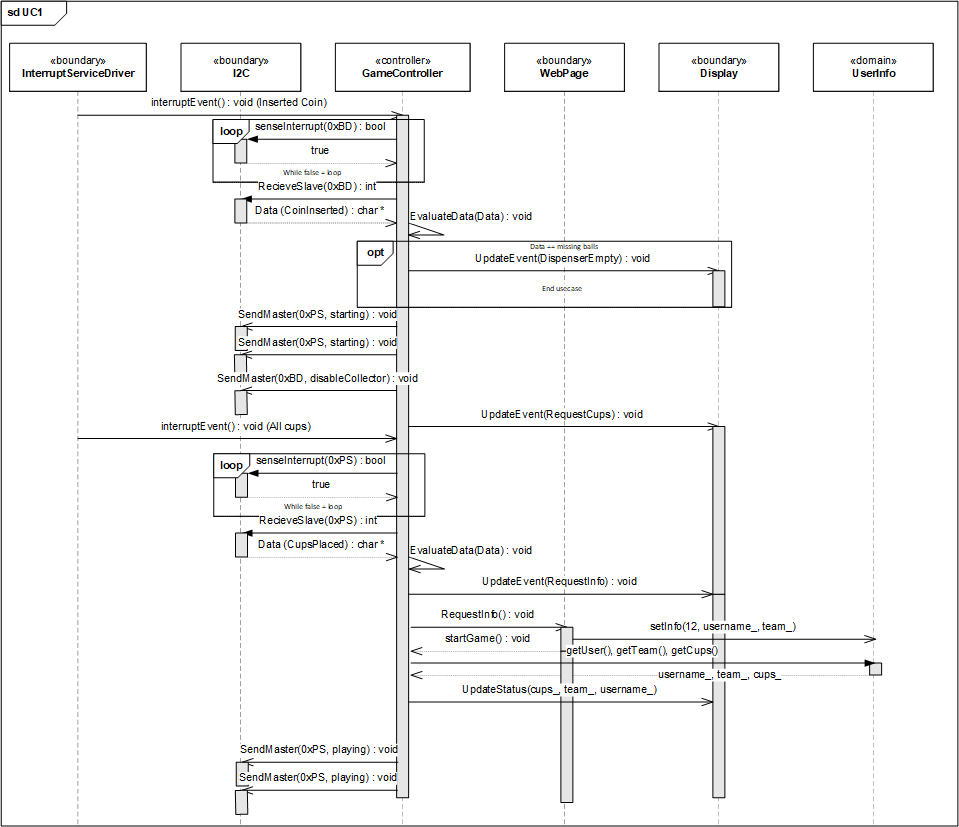
\includegraphics[width=\textwidth]{Arkitektur/Softwarearkitektur/Applikationsmodel/RPi/graphics_RPi/UC1_SD.png}
    \caption{Sekvensdiagram for UC1}
    \label{fig:UC1_SD_RPi}
\end{figure}

\textbf{Sekvensdiagram for UC2: GameController}\\
Spillet er startet og GameController har til opgave at hele tiden holde systemet opdateret i forhold til brugerens interaktioner. Hver gang brugeren fjerner en kop modtager RPi'en et interrupt fra Playerside-systemet. Denne information opbevares i UserInfo objekterne, således at både GameController og Displayet har adgang til hvilke kopper, som er placeret. 
\begin{figure}[H]
    \centering
    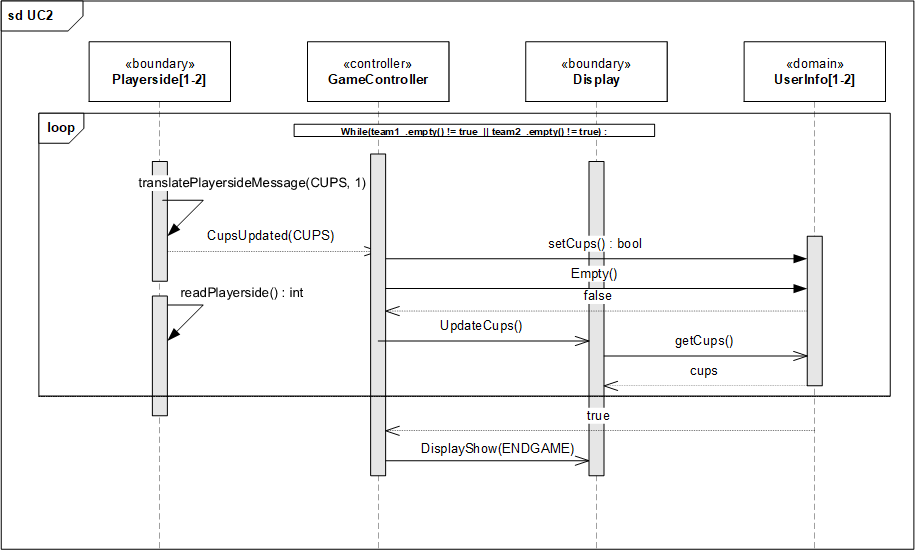
\includegraphics[width=\textwidth]{Arkitektur/Softwarearkitektur/Applikationsmodel/RPi/graphics_RPi/UC2_SD.png}
    \caption{Sekvensdiagram for UC2}
    \label{fig:UC2_SD_RPi}
\end{figure}

\newpage
\textbf{Sekvensdiagram for UC3: GameController}\\
GameControlleren har selv kontrolleret antallet af kopper tilbage på hvert side i forhold til det data, som har været sendt fra de to Playersides (Via UserInfo objekterne team1\_ og team2\_. Når den sidste kop er fjernet, sender den henholdsvis et signal til hver Playerside, i forhold til hvem som har vundet og tabt. Dette vises på displayet i et specifikt tidsinterval, hvor derefter systemet vil gå i dvale og være klar til nye spillere - GameController intiere stadiet "IDLE" til sidst, og giver samme besked til boundary klasserne. 

\begin{figure}[H]
    \centering
    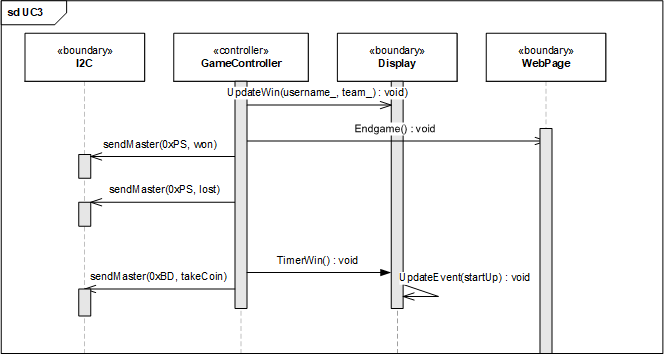
\includegraphics[width=\textwidth]{Arkitektur/Softwarearkitektur/Applikationsmodel/RPi/graphics_RPi/UC3_SD.png}
   \caption{Sekvensdiagram for UC3}
    \label{fig:UC3_SD_RPi}
\end{figure}

\newpage
\textbf{Sekvensdiagram for UC4: GameController}\\
I tilfælde af at BallDispenseren ikke har flere bolde, skal RPi'en udstede en besked til servicemedhjælperen og vente på at den er fyldt op (Eller har nok bolde til et spil). Når GameController modtager signalet "NotEmpty" fra BallDispenser kan den initiere stadiet "IDLE" igen. 

\begin{figure}[H]
    \centering
    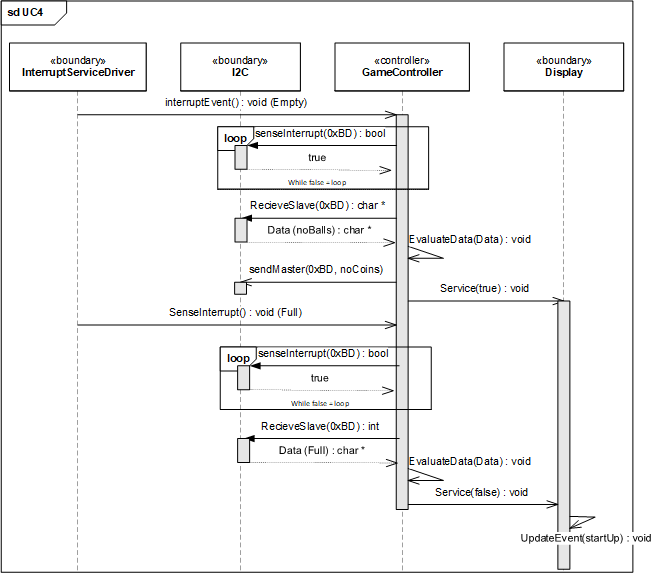
\includegraphics[width=\textwidth]{Arkitektur/Softwarearkitektur/Applikationsmodel/RPi/graphics_RPi/UC4_SD.png}
   \caption{Sekvensdiagram for UC4}
    \label{fig:UC4_SD_RPi}
\end{figure}

\textbf{Tilstandsmaskine: Display}\\
Displayet viser konstant spillets status og fortæller brugerne hvad de skal gøre. Den skifter derved også tilstand i takt med spillets gang. 

\begin{figure}[H]
    \centering
    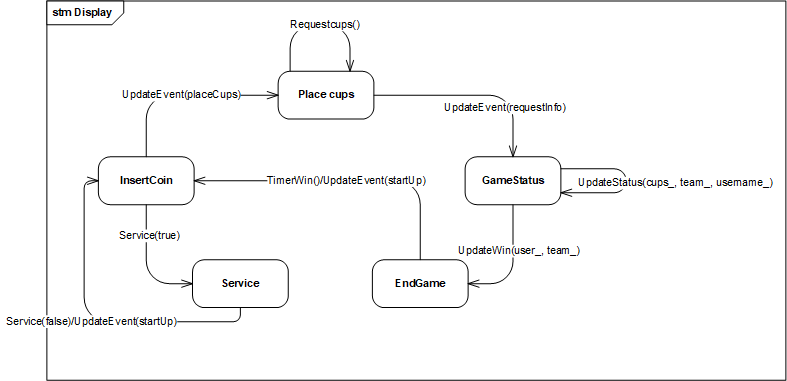
\includegraphics[width=\textwidth]{Arkitektur/Softwarearkitektur/Applikationsmodel/RPi/graphics_RPi/stm_disp.png}
    \caption{Tilstandsmaskine for Display}
    \label{fig:stm_disp}
\end{figure}

\textbf{Tilstandsmaskine: GameController}\\
Tilstandsmaskinen for GameController afspejler spillets gang. GameController skifter tilstand i forhold til de input den får givet fra PSOC-enhederne. Når den går ind i en given tilstand notificerer den alle boundary klasserne om dets tilstandsskifte - dette symboliseres ved funktionerne "SystemPlaying()", "SystemIdle()" osv. \\\\
GameController afspejler også hele systemets tilstand:
\begin{enumerate}
    \item IDLE: Send "IDLE"-tilstandsbesked til Playersides. Åben for møntmodtageren, tænd for displayet og vis tilhørende skærmbillede. 
    \item STARTING: Send "STARTING"-tilstandsbesked til Playersides. Luk for møntmodtager og vis tilhørende skærmbillede på displayet. Skal håndtere information om ny kop placering fra Playersides. Skal vente på bruger data fra WebPage. 
    \item PLAYING: Send "PLAYING"-tilstandsbesked til Playersides, samt "MyColor" og "OpponentColor". Vis tilhørende skærmbillede på displayet. Skal håndtere information om ny kop fra Playersides, samt indikere til displayet, hvornår en kop bliver fjernet / indsat. 
    \item ENDGAME: Send "LOST"- og "WON"-tilstandsbesked til Playesrsides. Vis tilhørende skærmbillede. Efter tidsinterval skal den initiere IDLE-tilstand. 
\end{enumerate}
\begin{figure}[H]
    \centering
    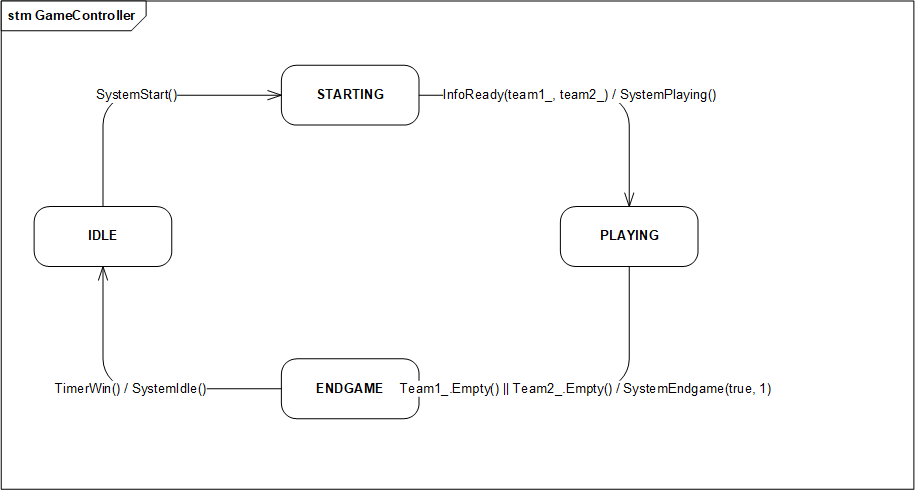
\includegraphics[width=\textwidth]{Arkitektur/Softwarearkitektur/Applikationsmodel/RPi/graphics_RPi/Stm_Game.png}
    \caption{Tilstandsmaskine for GameController}
    \label{fig:stm_Game}
\end{figure}

\textbf{Tilstandsmaskine: Refill Balls}\\
Denne tilstandsmaskine er forholdsvis simpel, og kan ses som en forlængelse af GameControllers - den er blot delt op for at gøre det mere overskueligt. Hvis RPi'en modtager informationen, at der er mangle på bolde "EMPTY", så initiere den tilstanden "SERVICE": 
\begin{enumerate}
    \item SERVICE: Luk for møntmodtageren, og vis tilhørende skærmbillede (Hidkald servicemedhjælper). Vent indtil bolddispenseren er påfyldt 2 eller flere bolde og har sendt beskeden "NOTEMPTY". 
\end{enumerate}

%%MANGLER BILLEDE!

\end{document}